\chapter{Изменение точек для вихревого поля скоростей (lagrangian)}
\label{app:vortex_lg}

\begin{figure}[h]
	\centering
	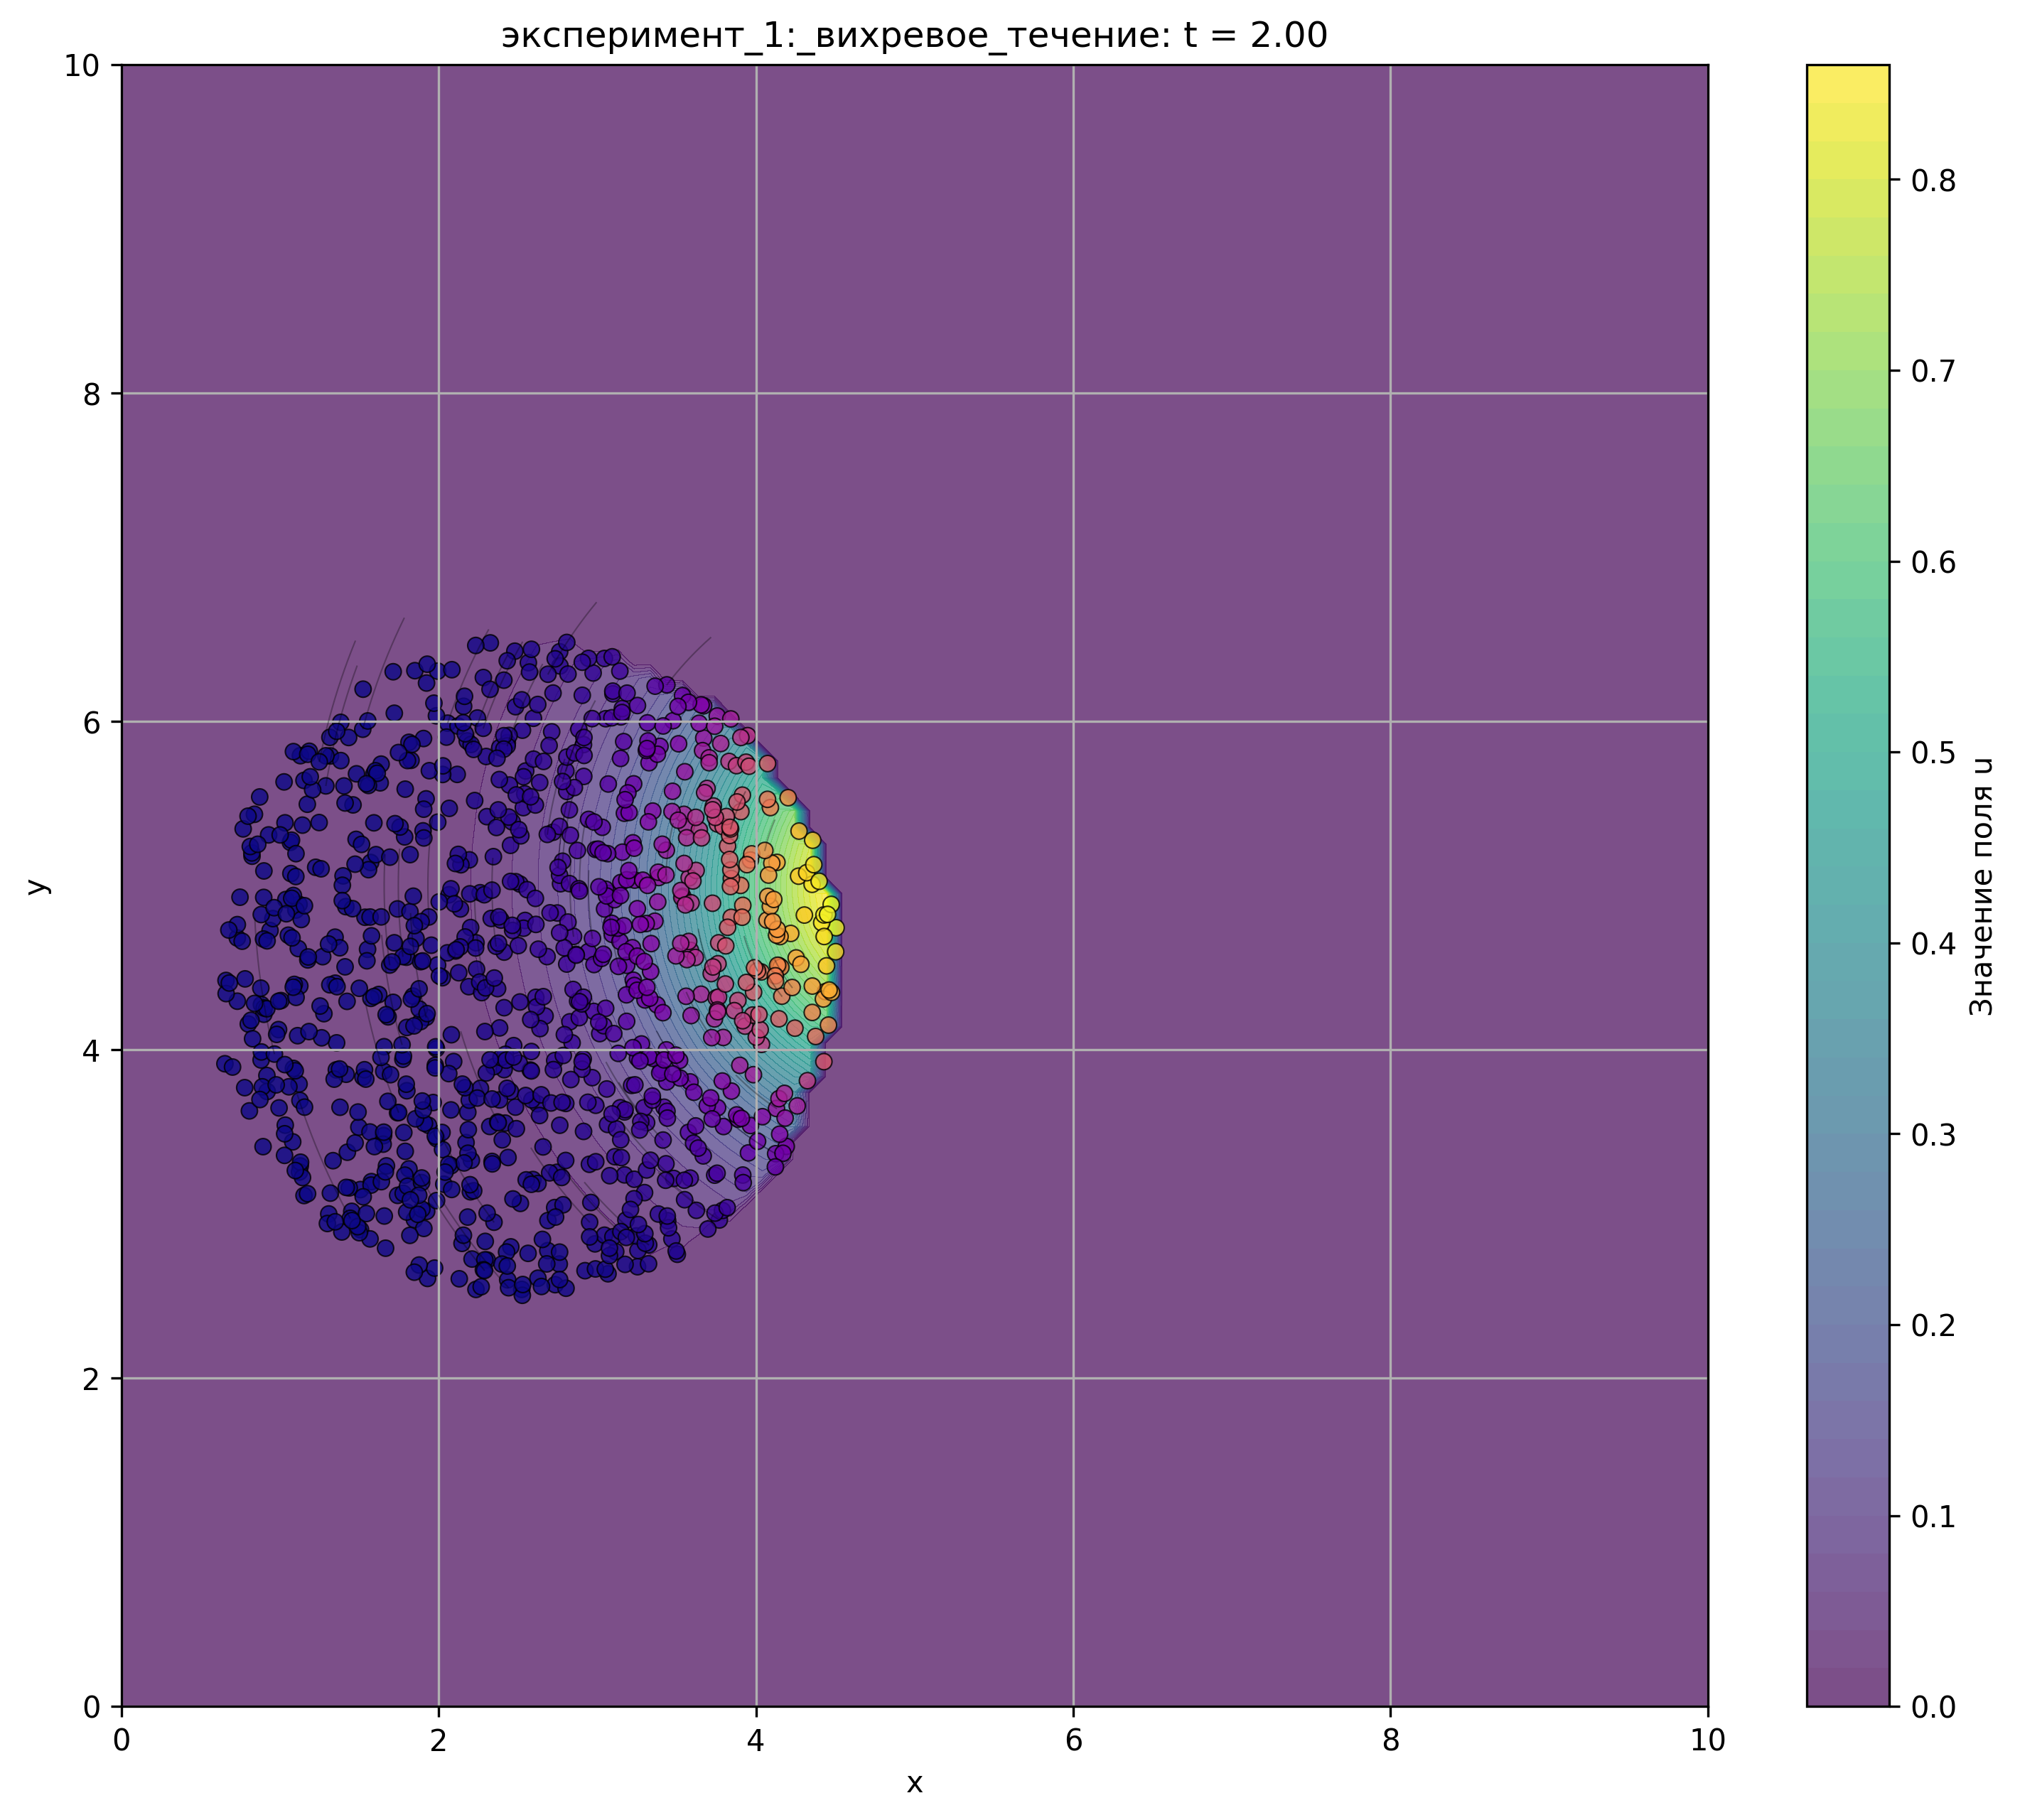
\includegraphics[width=0.6\textwidth]{imgs/lg/эксперимент_1:_вихревое_течение_t2.00.png}
	\caption{Скалярное поле в момент времени $t=2$ }
\end{figure}
\begin{figure}[h]
	\centering
	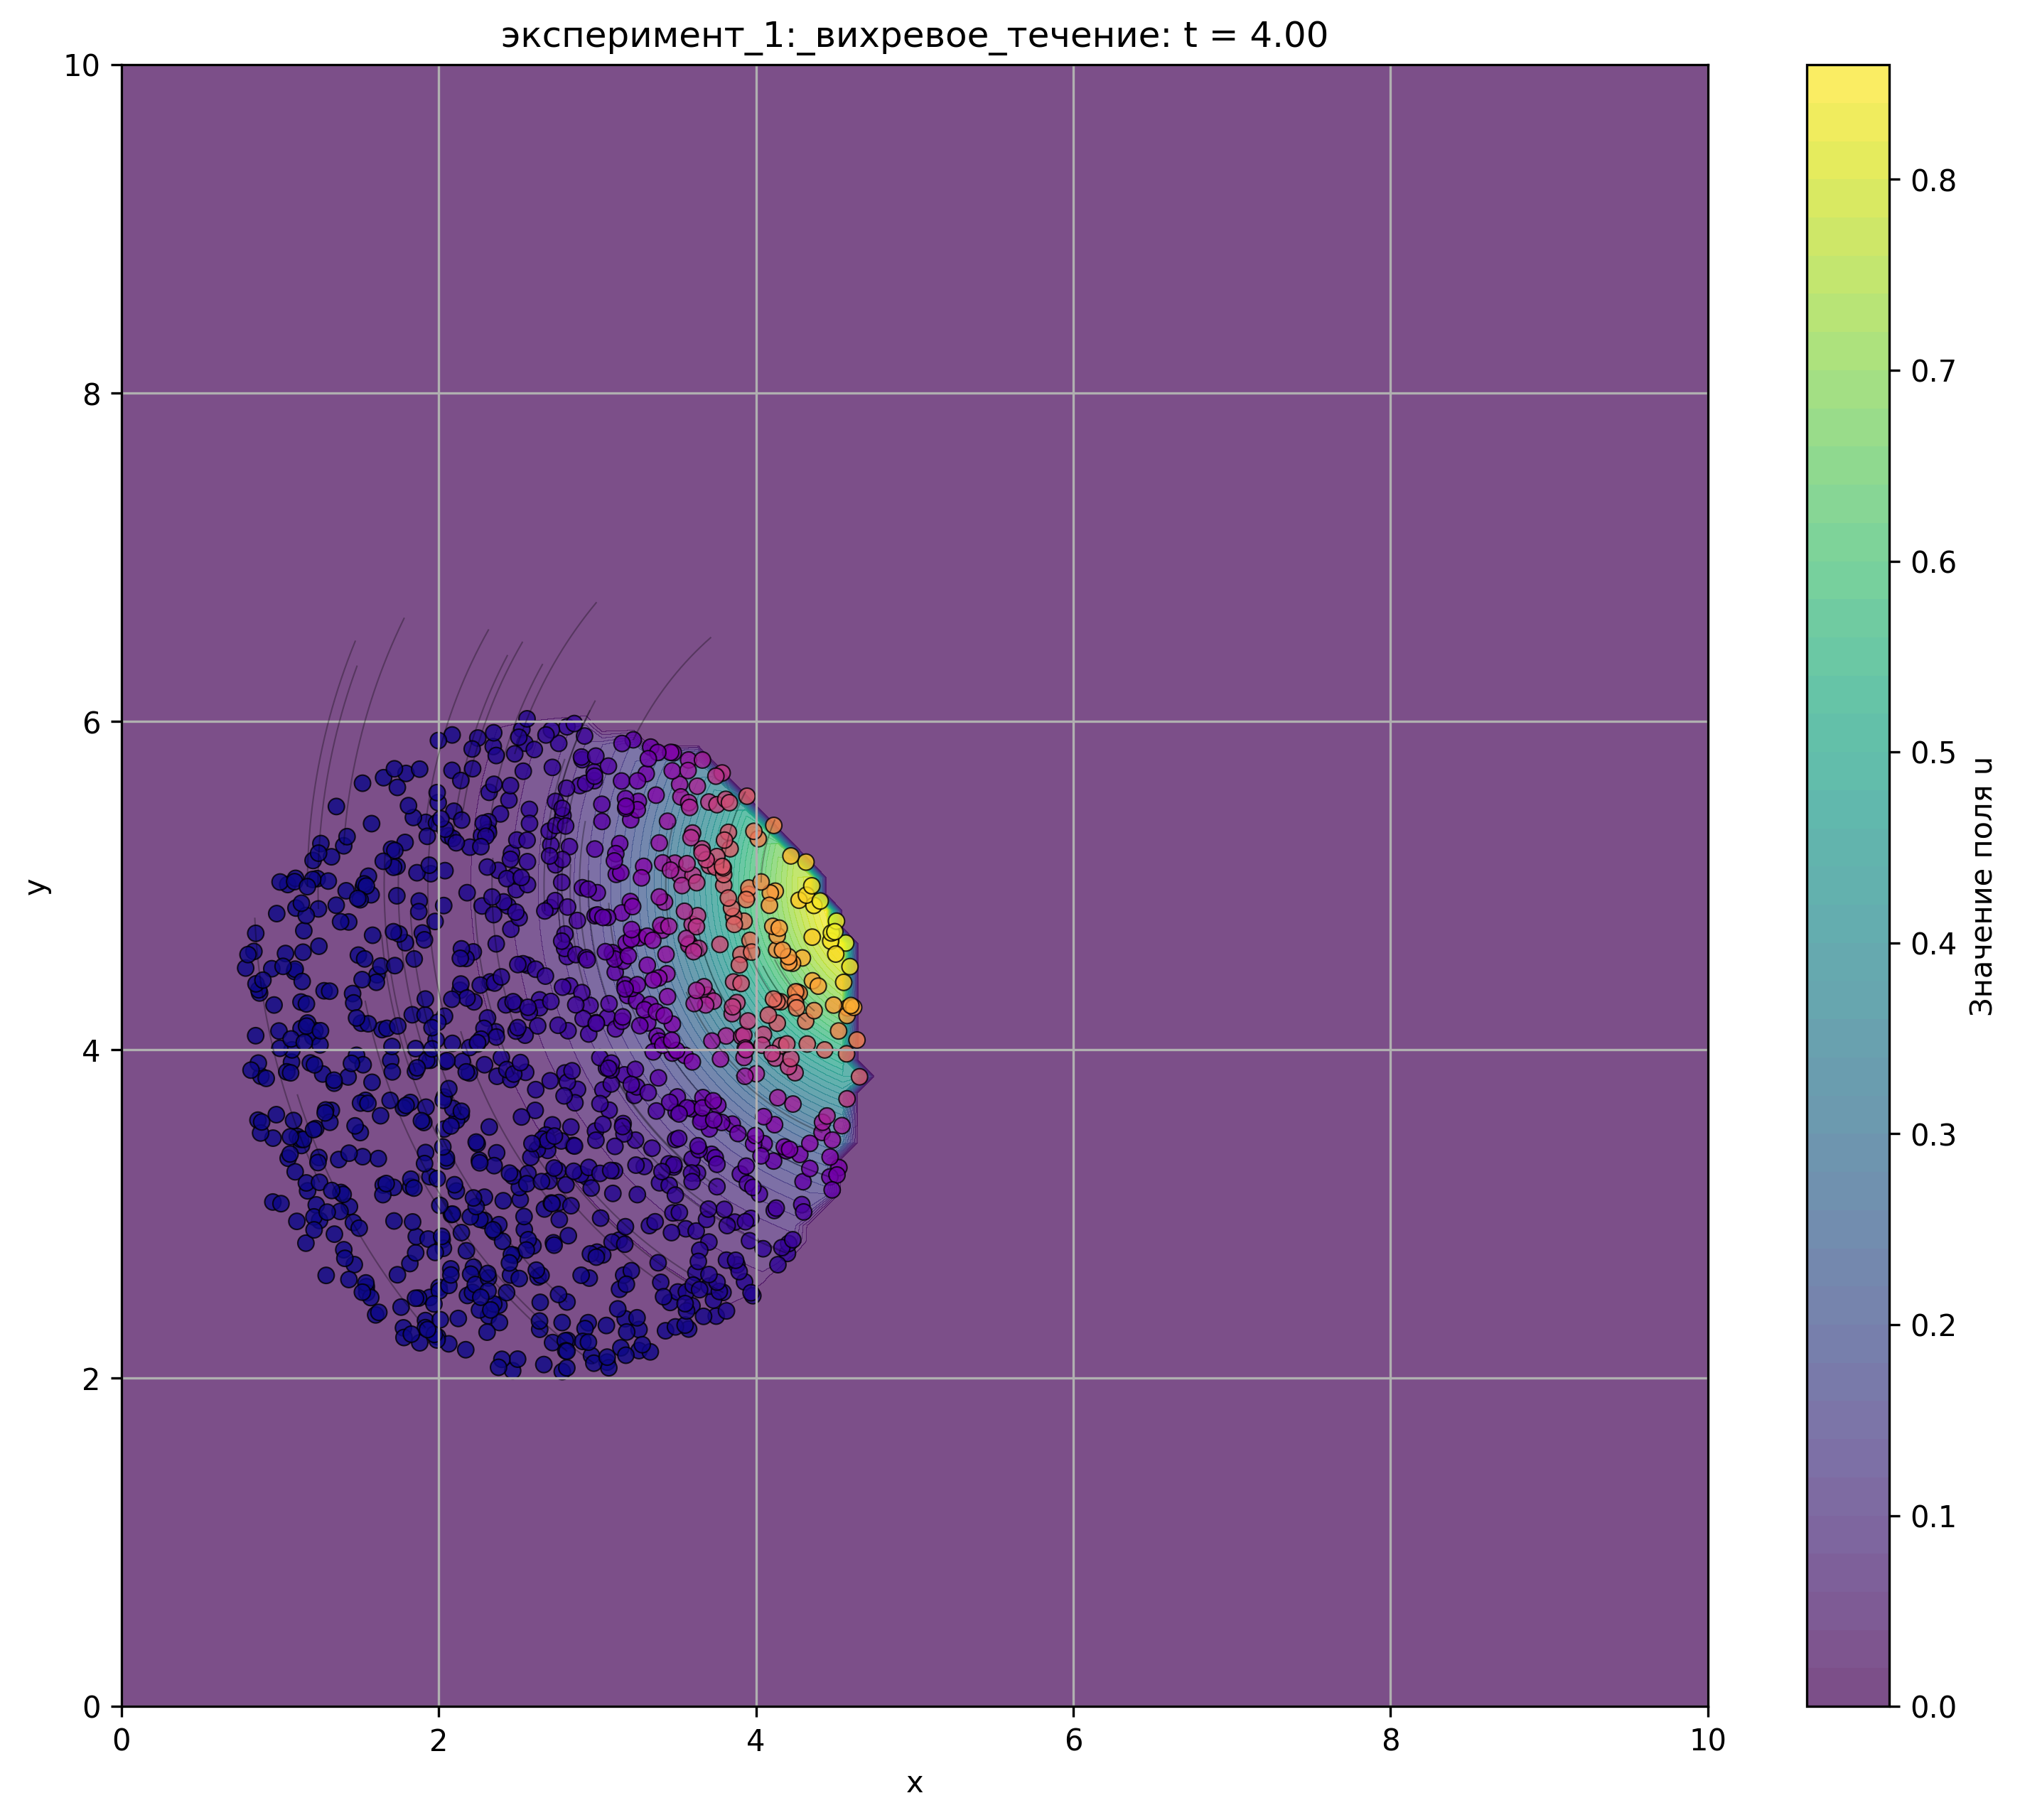
\includegraphics[width=0.6\textwidth]{imgs/lg/эксперимент_1:_вихревое_течение_t4.00.png}
	\caption{Скалярное поле в момент времени $t=4$ }
\end{figure}
\begin{figure}[h]
	\centering
	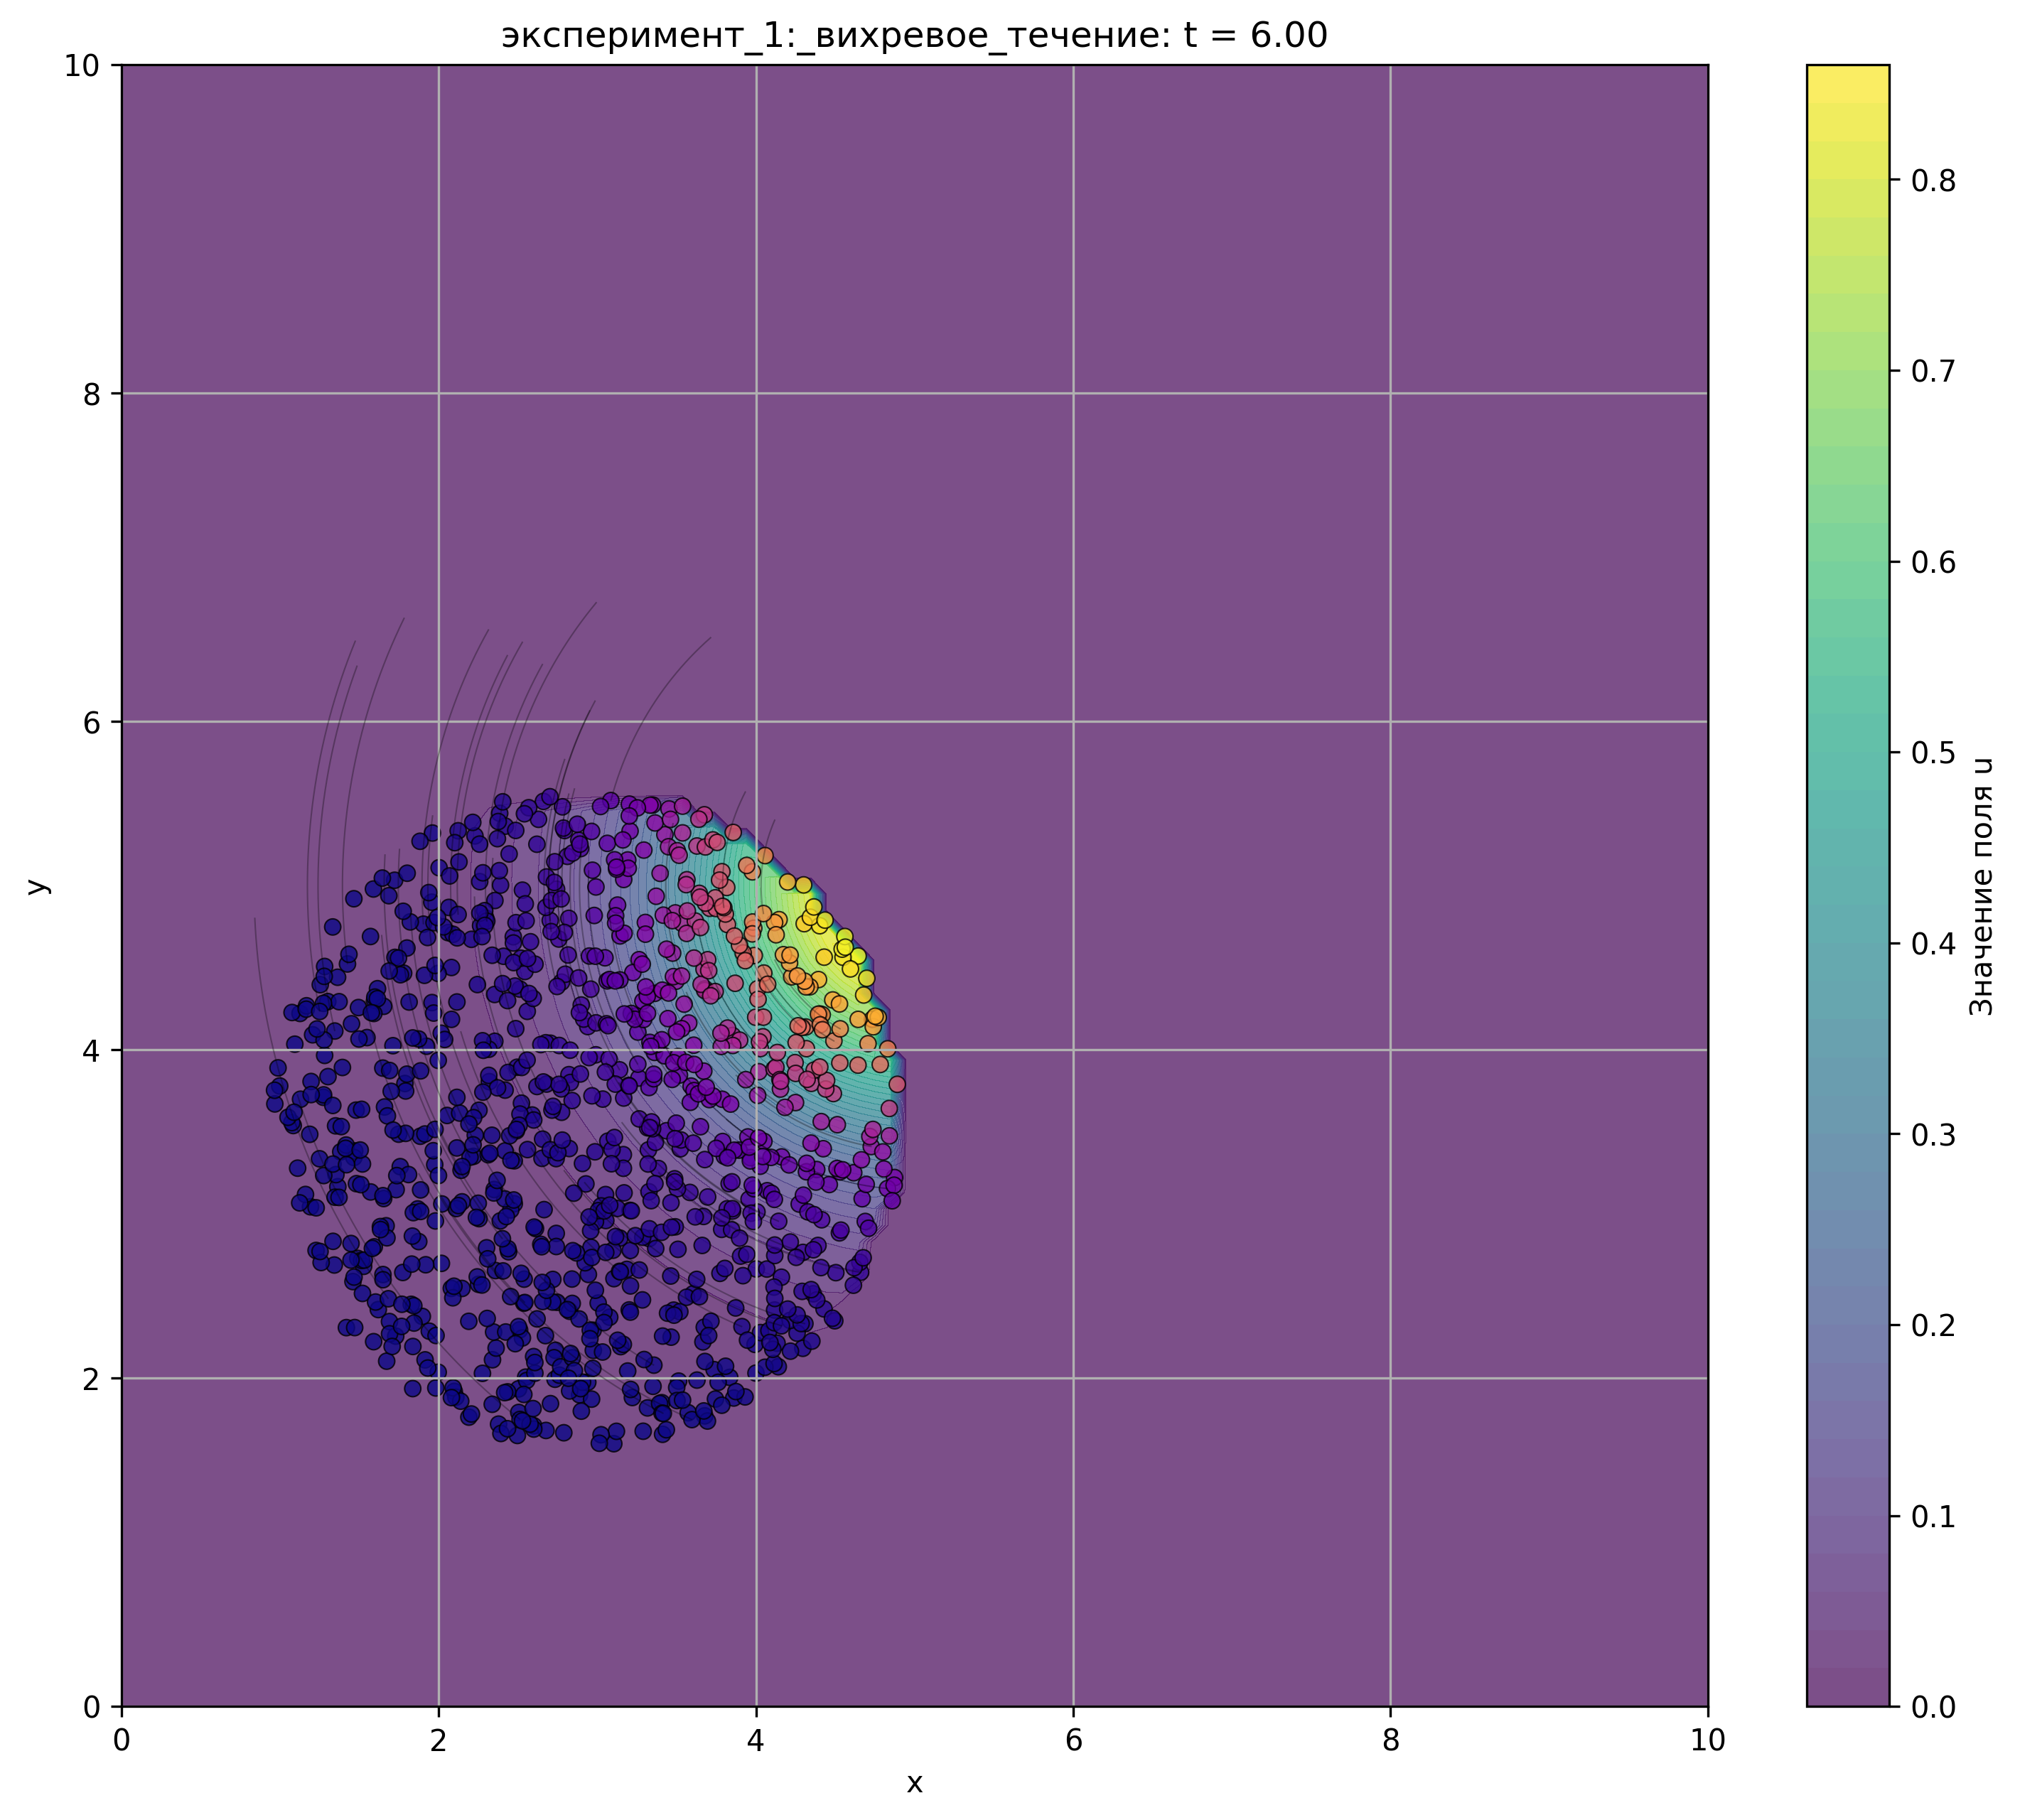
\includegraphics[width=0.6\textwidth]{imgs/lg/эксперимент_1:_вихревое_течение_t6.00.png}
	\caption{Скалярное поле в момент времени $t=6$ }
\end{figure}
\begin{figure}[h]
	\centering
	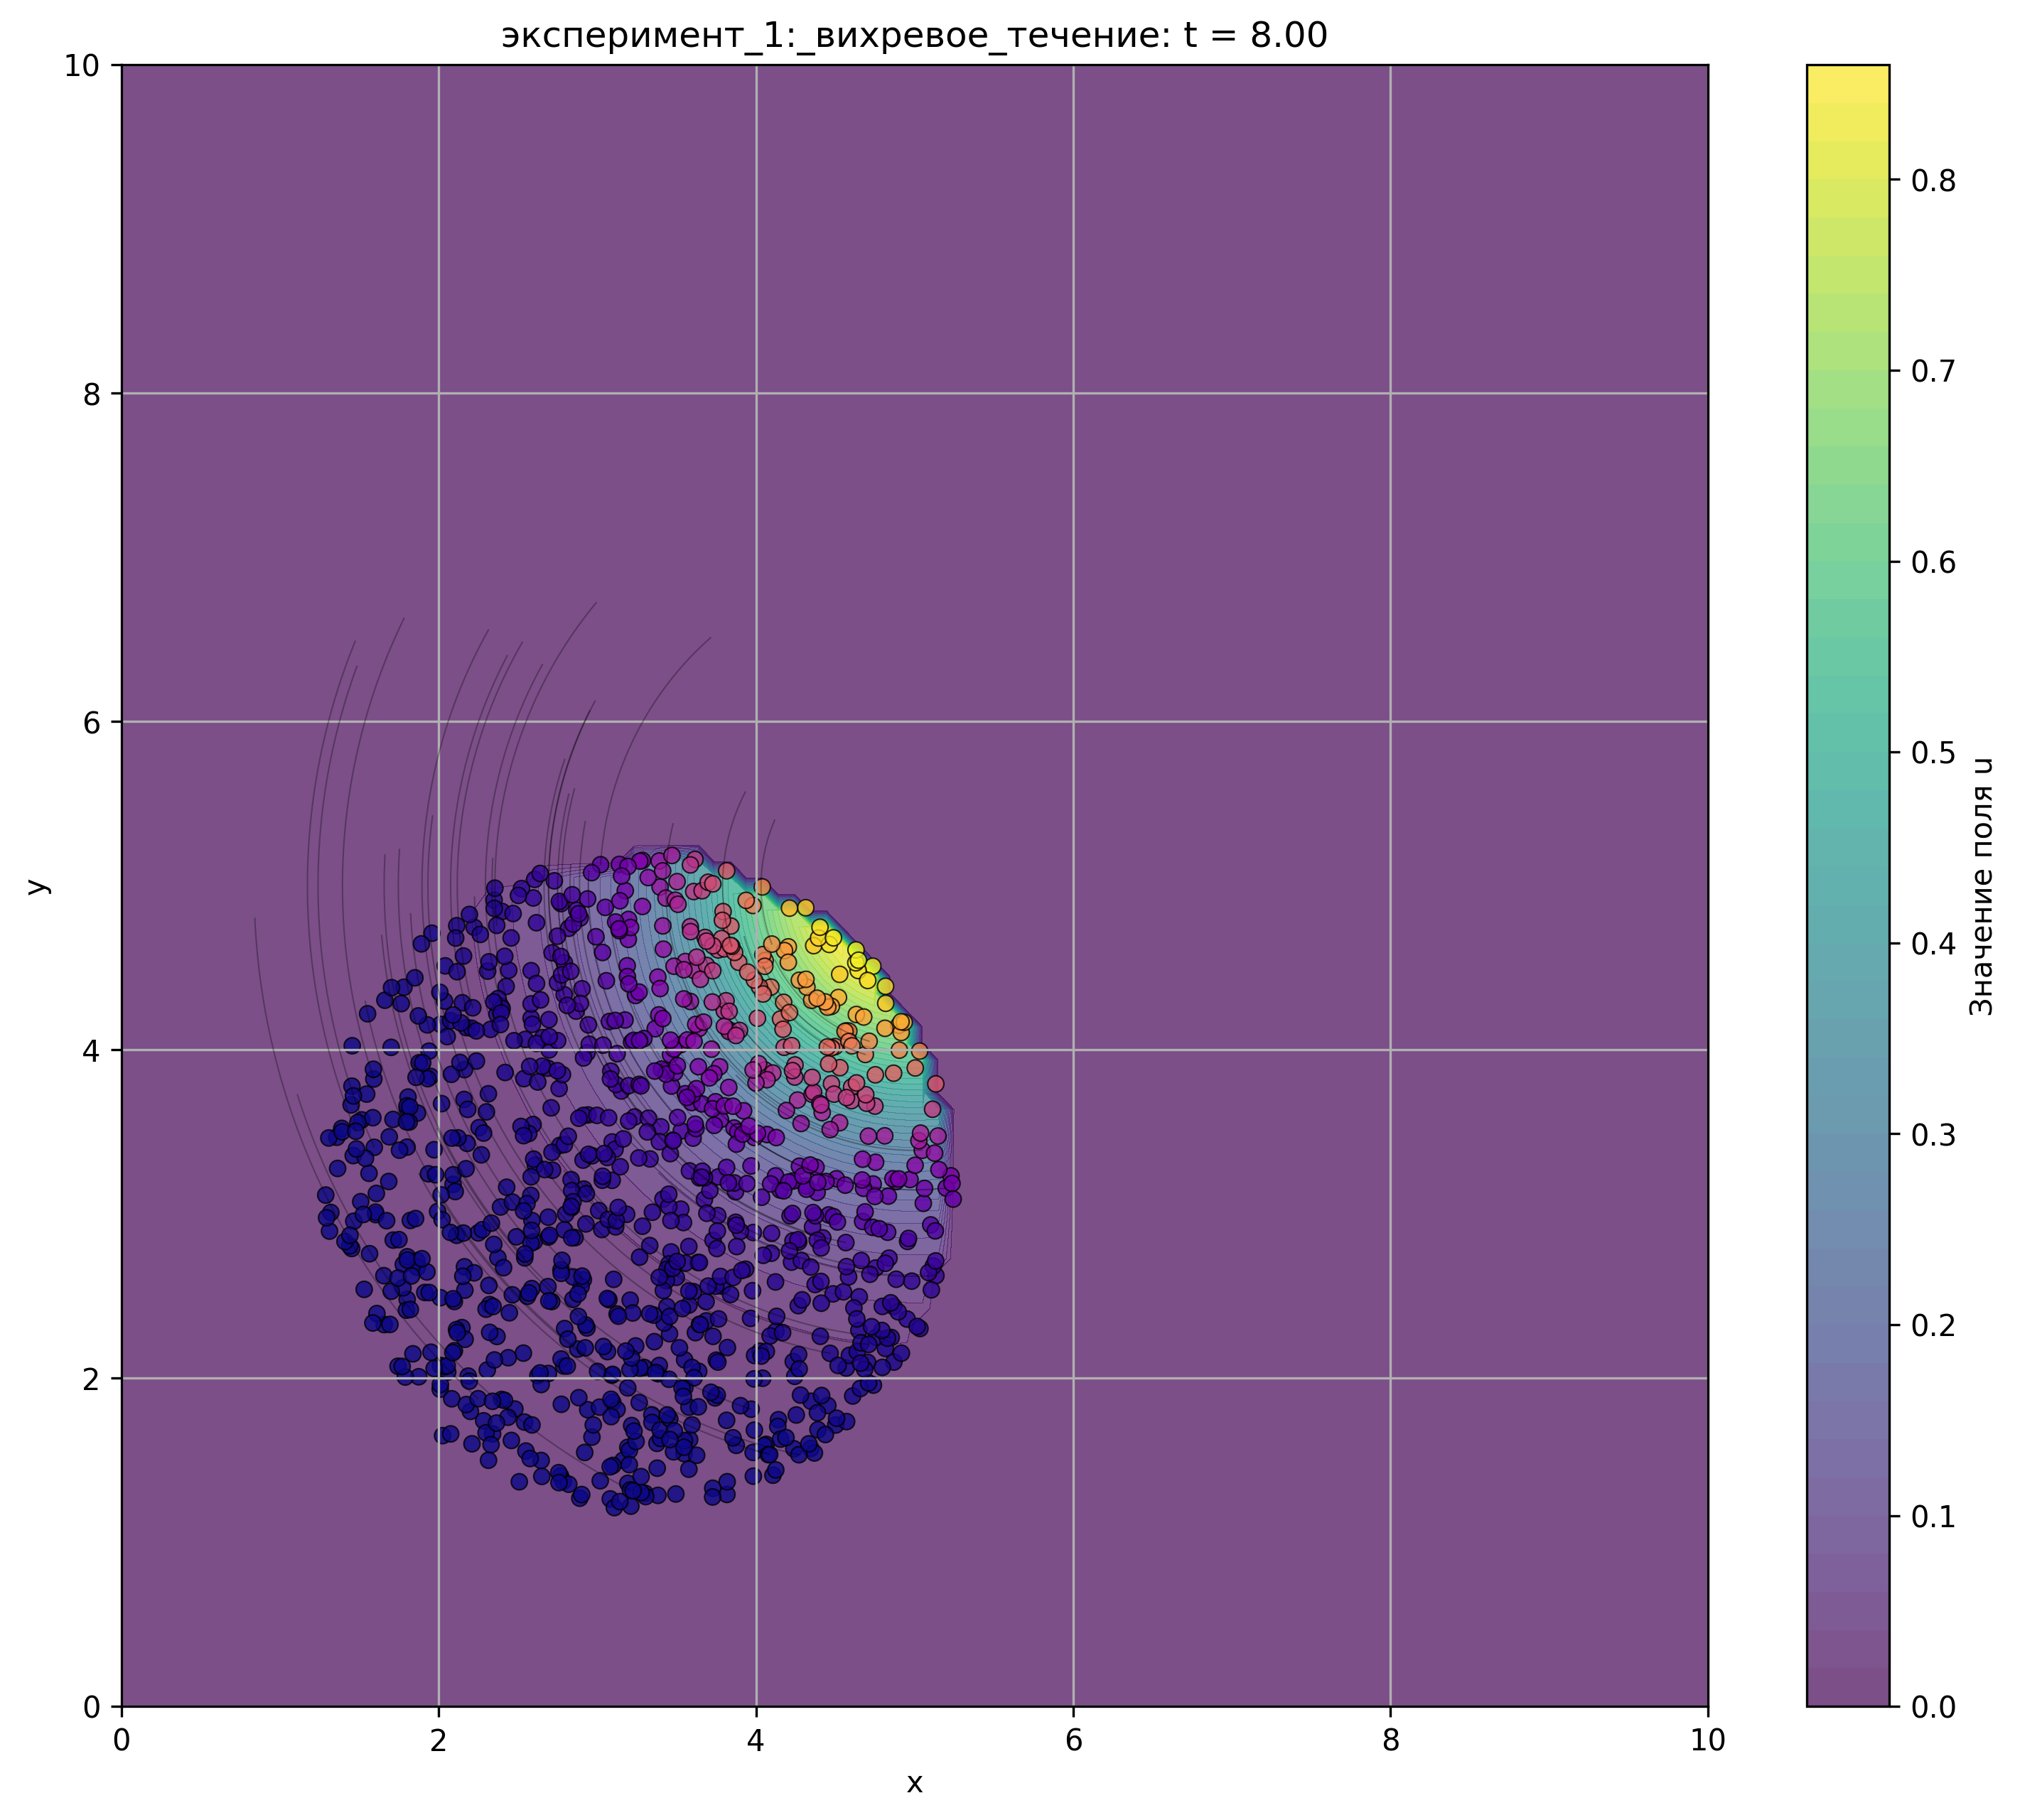
\includegraphics[width=0.6\textwidth]{imgs/lg/эксперимент_1:_вихревое_течение_t8.00.png}
	\caption{Скалярное поле в момент времени $t=8$ }
\end{figure}